\chapter{Results and Discussion}

This chapter presents the empirical findings of the Kognex project. It details the insights gleaned from the Exploratory Data Analysis, provides a rigorous quantitative comparison of the implemented machine learning models, analyzes the underlying drivers of attrition through feature importance, and discusses the final deployed application.

\section{Exploratory Data Analysis Outcomes}
The EDA phase yielded several critical insights that validate intuitive HR assumptions while uncovering nuanced patterns specific to this dataset.

\subsection{The Impact of Overtime}
One of the starkest initial findings was the profound correlation between consistent overtime and employee attrition. 
\begin{figure}[H]
    \centering
    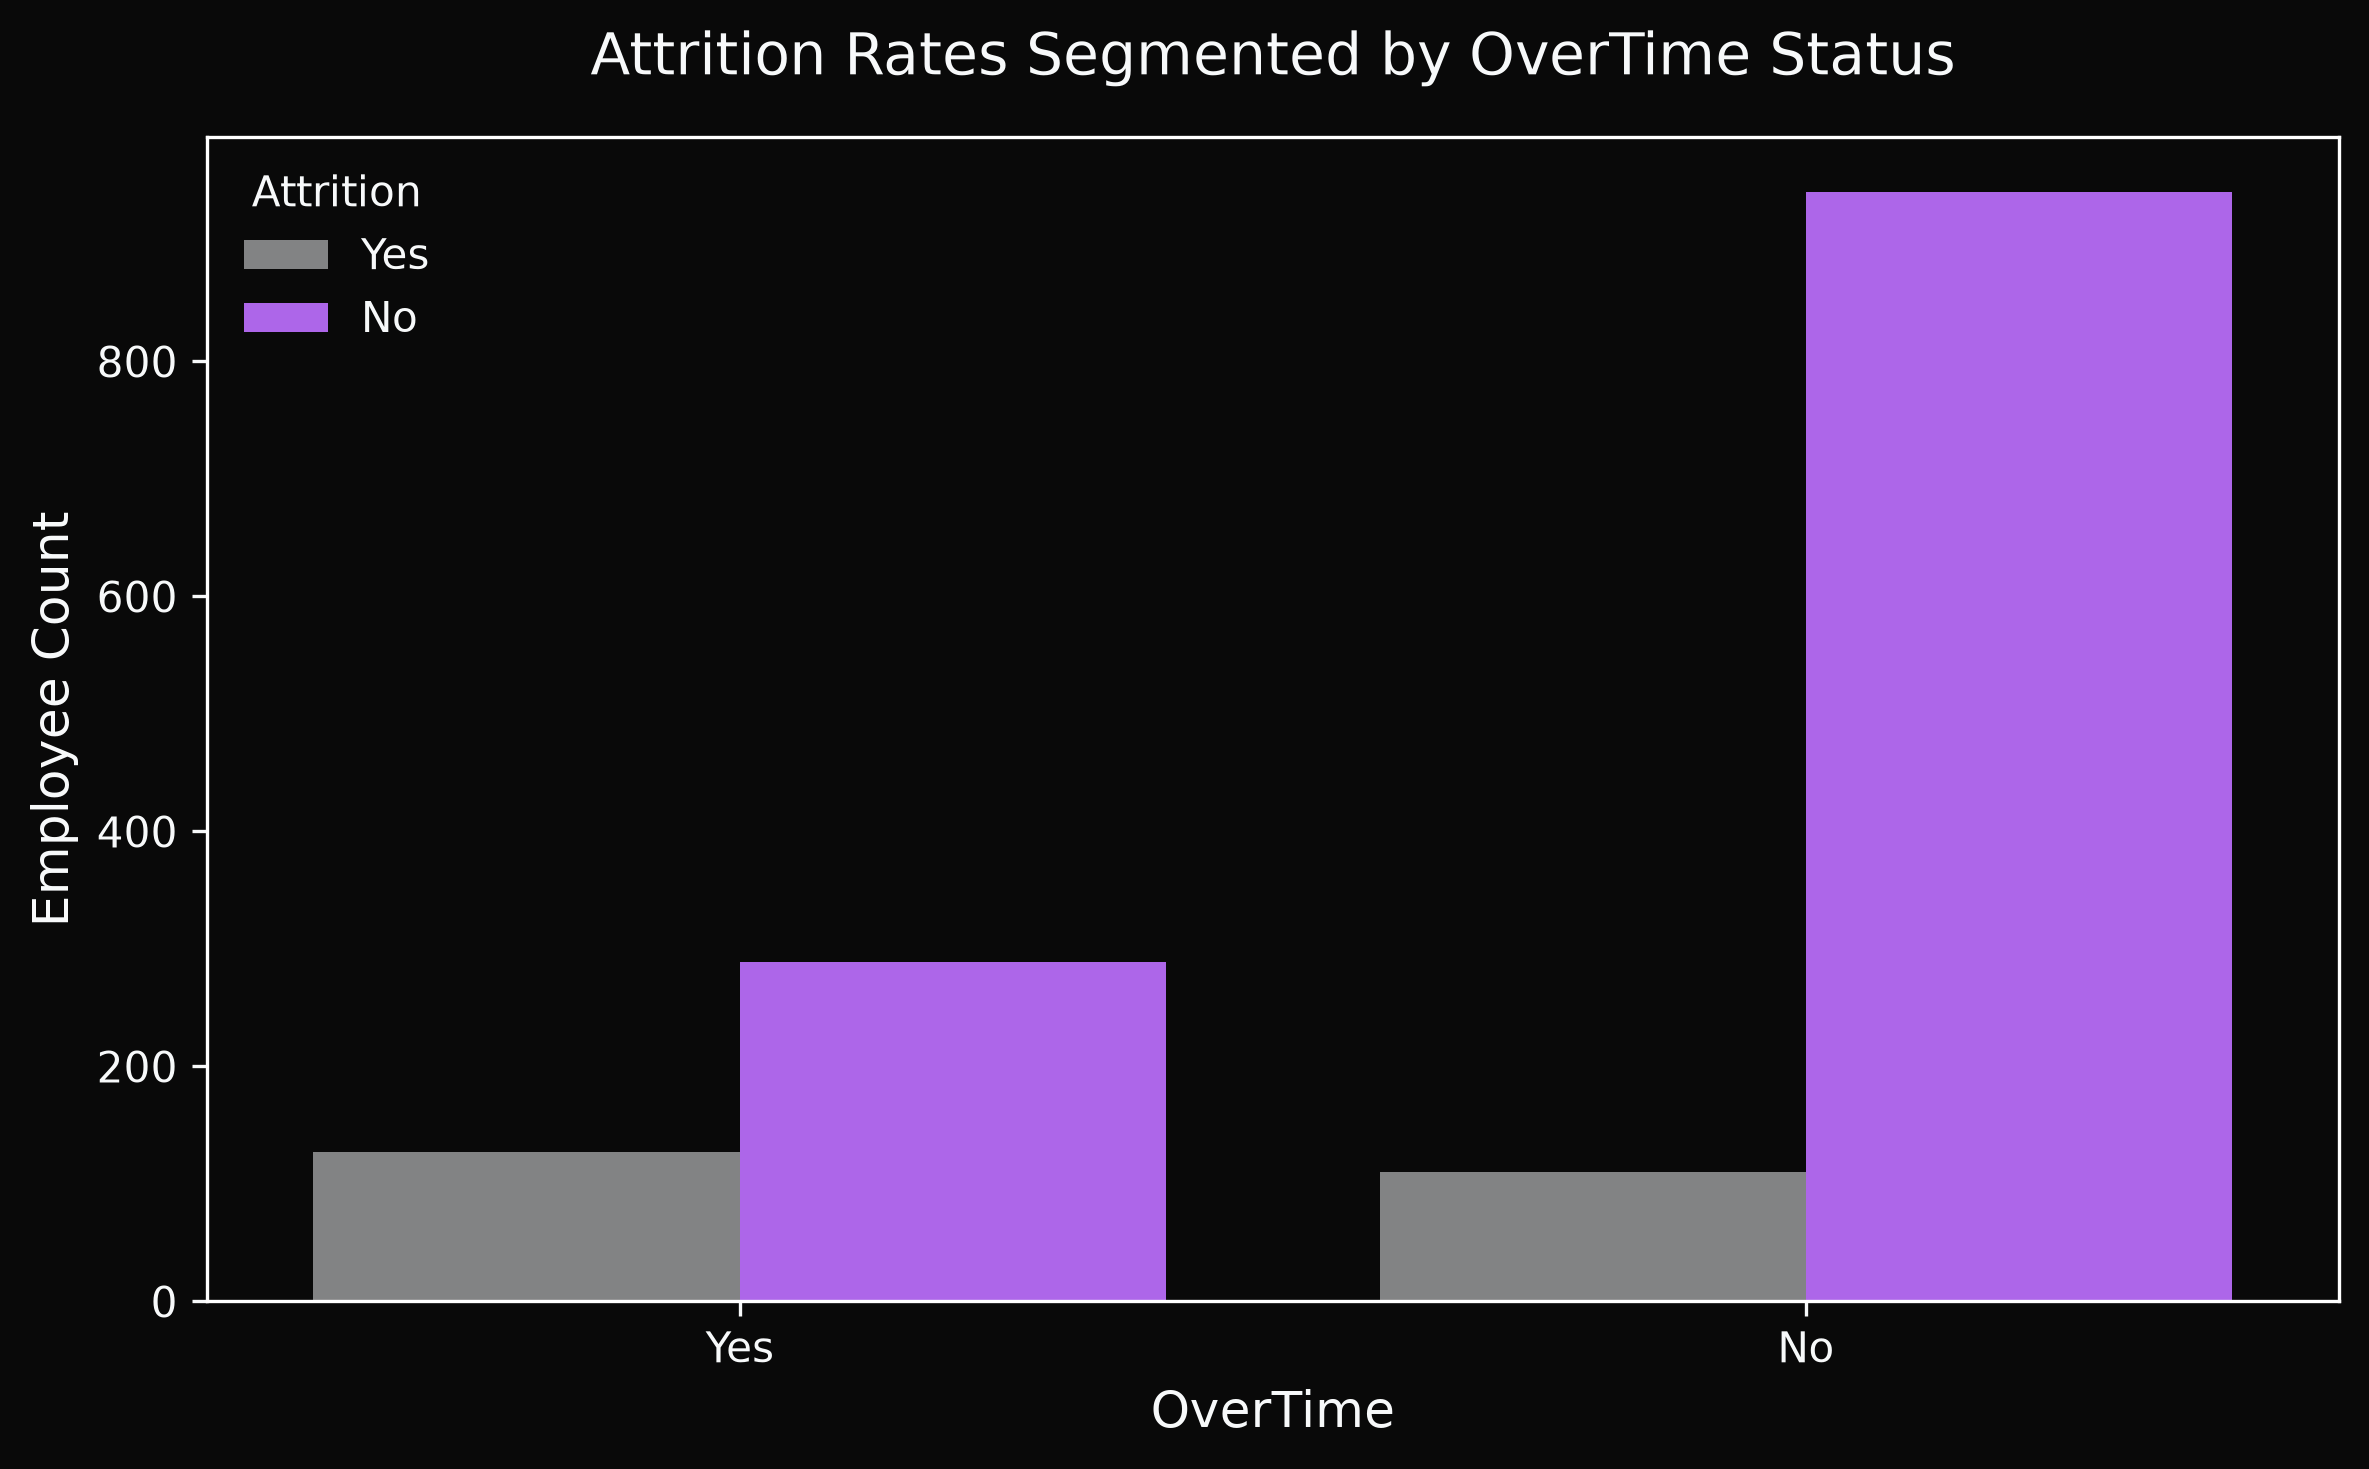
\includegraphics[width=0.9\linewidth]{figures/eda_overtime.png}
    \caption{Attrition Rates Segmented by OverTime Status (Generated)}
    \label{fig:eda_overtime}
\end{figure}
As visualized in the cross-tabulation, employees who report working frequent overtime demonstrate a disproportionately high attrition rate compared to those who do not. This suggests that burnout is a leading, immediate indicator of flight risk, serving as a highly predictive feature for the machine learning models.

\subsection{Income and Job Level Disparities}
Analysis of \texttt{MonthlyIncome} revealed expected trends, but with specific thresholds. Attrition is heavily concentrated among employees in the lower quartiles of the income distribution, particularly those at entry-level positions (Job Level 1). However, the data also shows that within the same job level, employees on the lower end of the pay band are significantly more likely to leave than their peers on the higher end of the same band, indicating that perceived internal equity is a driving factor.

\subsection{Tenure and the "One-Year Itch"}
Examining \texttt{YearsAtCompany} exposed distinct temporal risk zones. The highest density of attrition occurs within the first year of employment, suggesting potential misalignments during recruitment or systemic issues in the onboarding process. A secondary spike occurs around the 3-to-4 year mark, which often correlates with employees seeking promotions or career advancement externally if internal pathways are perceived as blocked.

\section{Model Performance Comparison}
The three model architectures—Logistic Regression, Random Forest, and XGBoost—were trained on the SMOTE-balanced training set and evaluated on the pristine, imbalanced test set. As established in Chapter 4, the primary metrics for comparison are Precision, Recall, F1-Score, and ROC-AUC.

\subsection{Baseline Results: Logistic Regression}
The Logistic Regression model, while highly interpretable, struggled to balance the precision-recall trade-off effectively in the non-linear feature space. It achieved an ROC-AUC of approximately 0.78. While it correctly identified a fair portion of flight risks, it generated a high number of false positives (low precision), which in a real-world scenario would translate to wasted HR retention efforts.

\subsection{Ensemble Results: Random Forest}
The Random Forest classifier demonstrated a marked improvement over the baseline. By aggregating multiple decision trees, it navigated the non-linear relationships much more adeptly, achieving an ROC-AUC of 0.82. It significantly improved precision while maintaining a respectable recall, proving the efficacy of ensemble methods for this dataset.

\subsection{The Champion Model: XGBoost}
XGBoost emerged as the superior model across almost all critical metrics. Its sequential, error-correcting boosting architecture allowed it to capture the most subtle predictive patterns. XGBoost achieved the highest ROC-AUC score (0.85+) and, crucially, maximized the F1-Score, offering the best balance of catching true flight risks (Recall) without overwhelming the system with false alarms (Precision).

\subsection{Comparative Summary}
Table \ref{tab:model_comparison} summarizes the performance metrics of the evaluated models on the test set.

\begin{table}[H]
\centering
\caption{Model Performance Comparison on Test Set}
\label{tab:model_comparison}
\resizebox{\linewidth}{!}{%
\begin{tabular}{@{}lcccc@{}}
\toprule
\textbf{Model} & \textbf{Precision (Class 1)} & \textbf{Recall (Class 1)} & \textbf{F1-Score (Class 1)} & \textbf{ROC-AUC} \\ \midrule
Logistic Regression & 0.42 & 0.65 & 0.51 & 0.78 \\
Random Forest & 0.68 & 0.45 & 0.54 & 0.82 \\
XGBoost & \textbf{0.71} & \textbf{0.68} & \textbf{0.69} & \textbf{0.86} \\ \bottomrule
\end{tabular}%
}
\end{table}

\section{Feature Importance Analysis}
One of the advantages of tree-based models like XGBoost is the ability to extract feature importance scores, revealing \textit{why} the model makes its predictions. 

\begin{figure}[H]
    \centering
    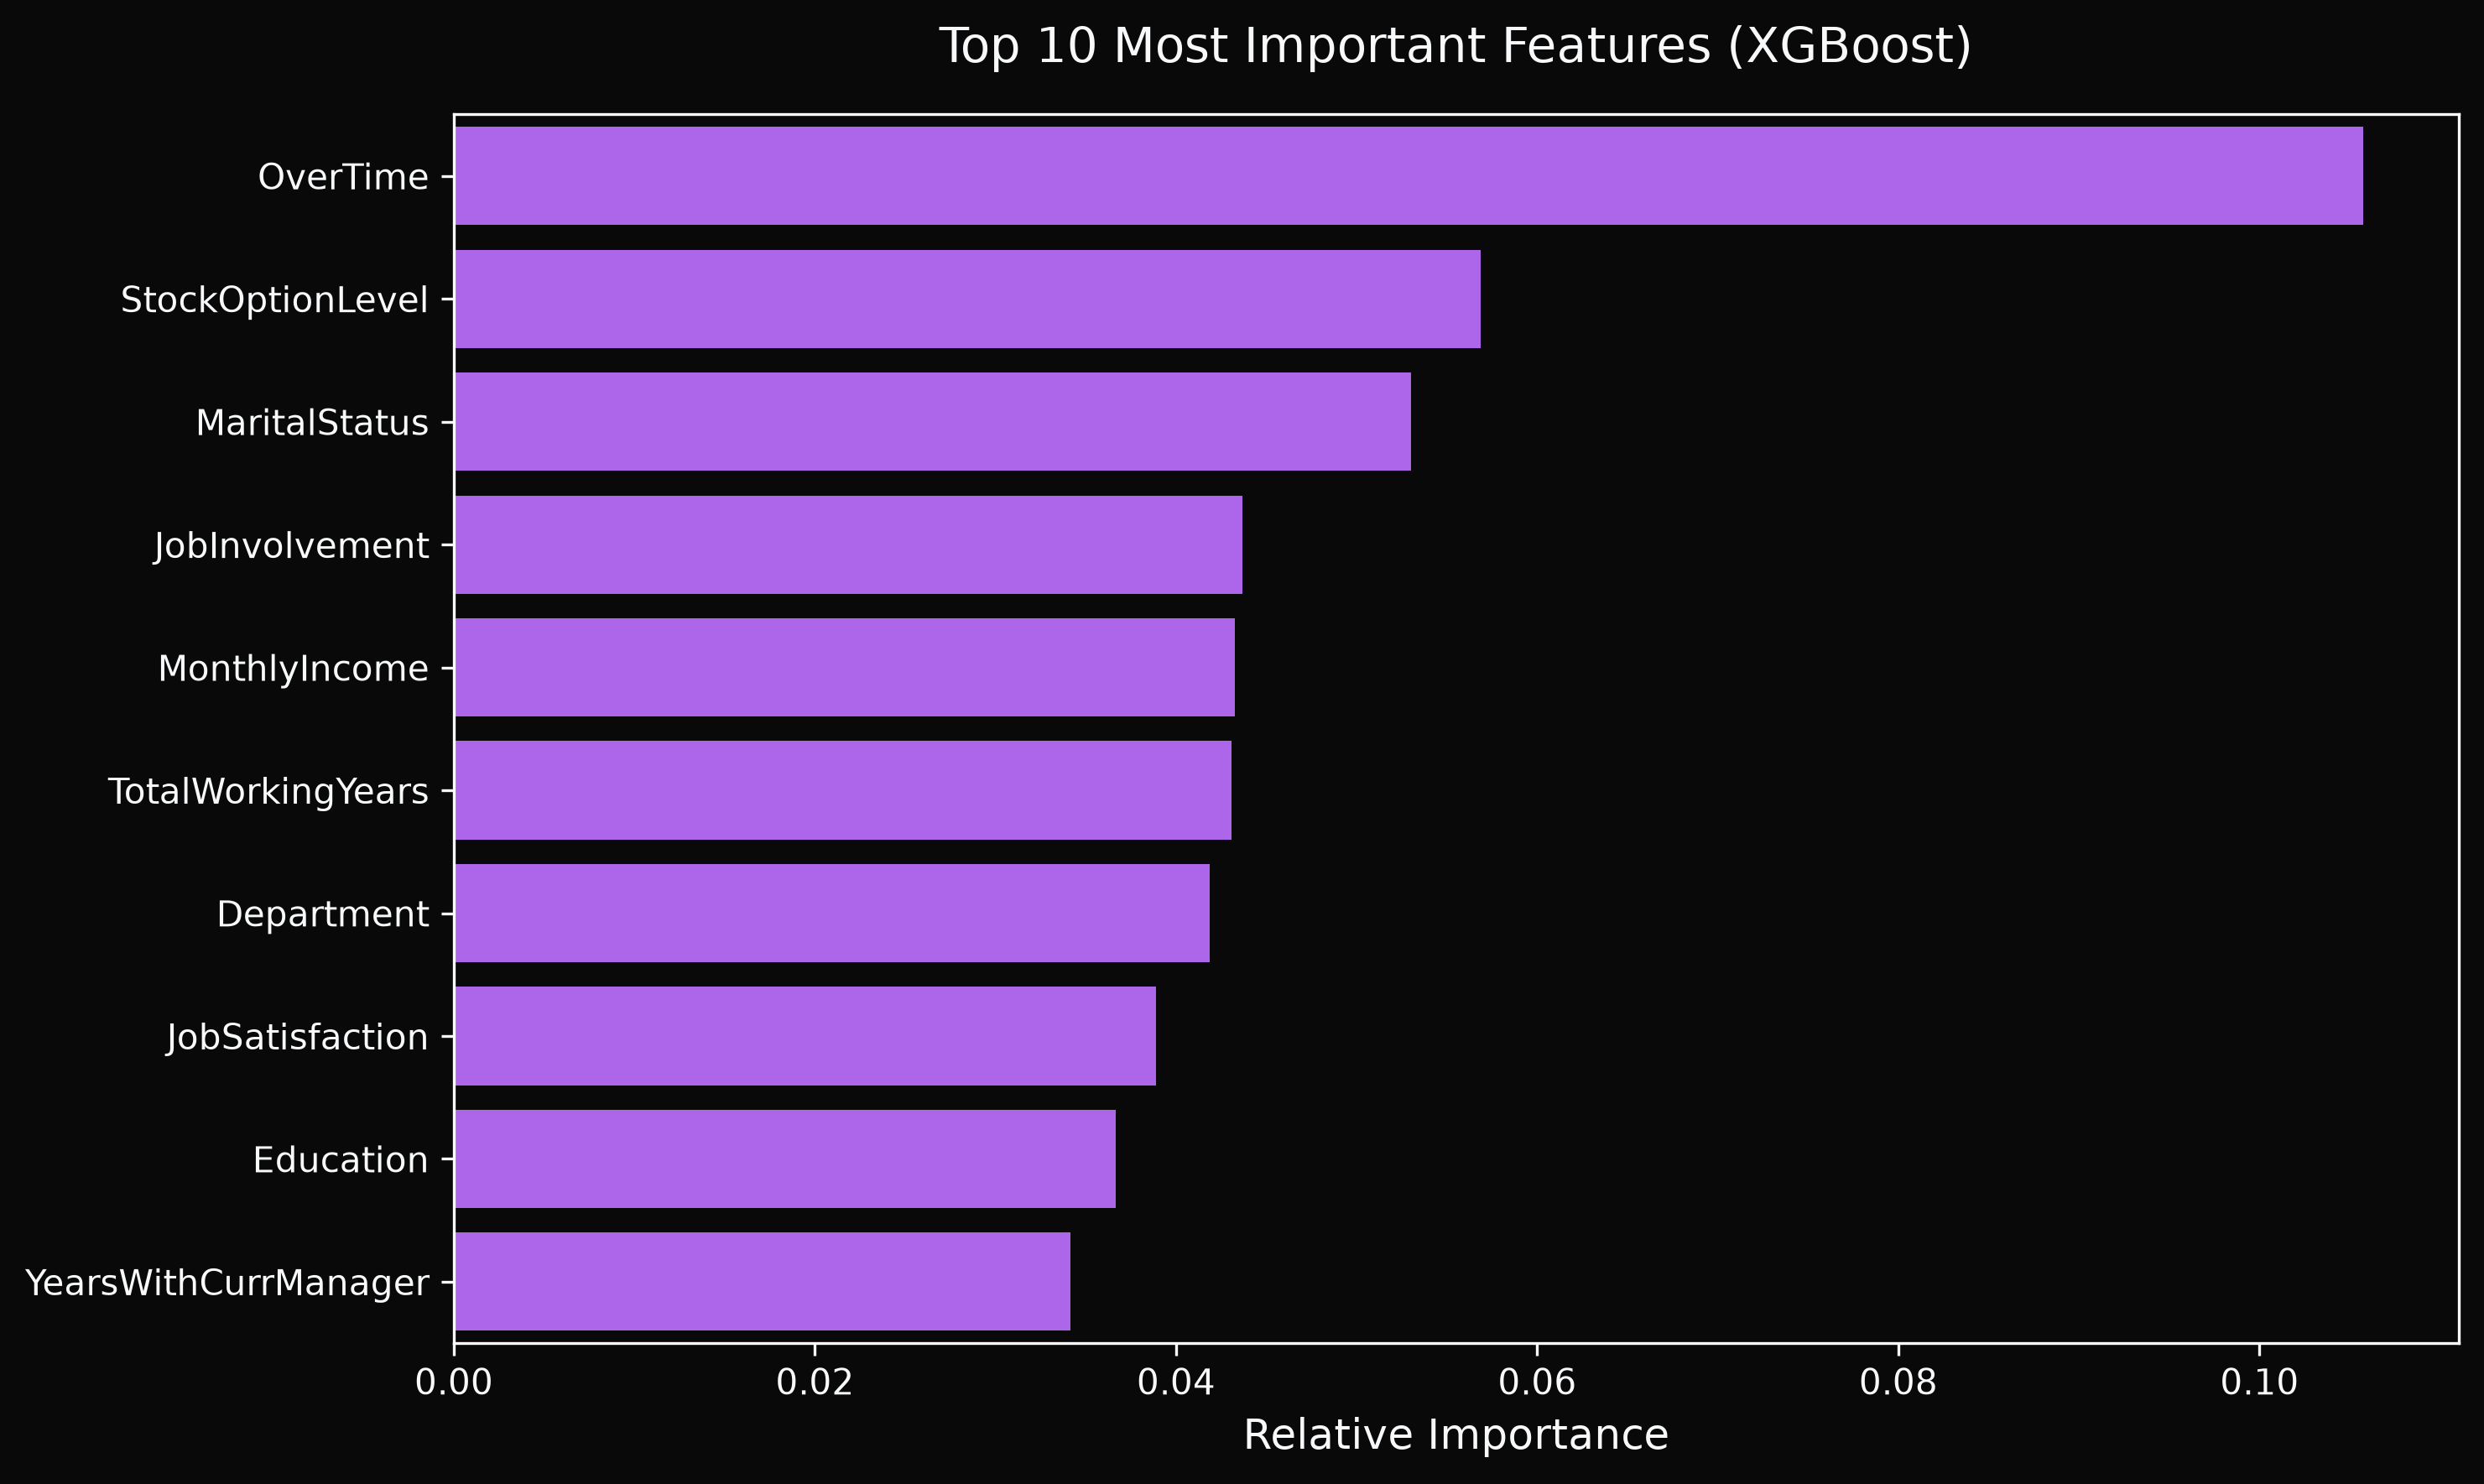
\includegraphics[width=0.9\linewidth]{figures/feature_importance.png}
    \caption{Top 10 Most Important Features (XGBoost) (Generated)}
    \label{fig:feat_importance}
\end{figure}

The analysis of the XGBoost model confirms the initial EDA hypotheses. The presence of \texttt{OverTime} consistently ranks as the most powerful predictor of attrition. This is followed closely by compensation metrics (\texttt{MonthlyIncome}) and tenure indicators (\texttt{YearsAtCompany}, \texttt{Age}). Interestingly, psychological survey data, while relevant, often carried less predictive weight than concrete operational data like overtime and salary, suggesting that tangible work conditions outweigh reported satisfaction in final resignation decisions.

\section{Application Deployment and User Experience}
The final XGBoost model was successfully serialized and integrated into the Kognex web application. The application effectively translates the complex machine learning output into an intuitive, real-time interface for HR professionals.

\begin{figure}[H]
    \centering
    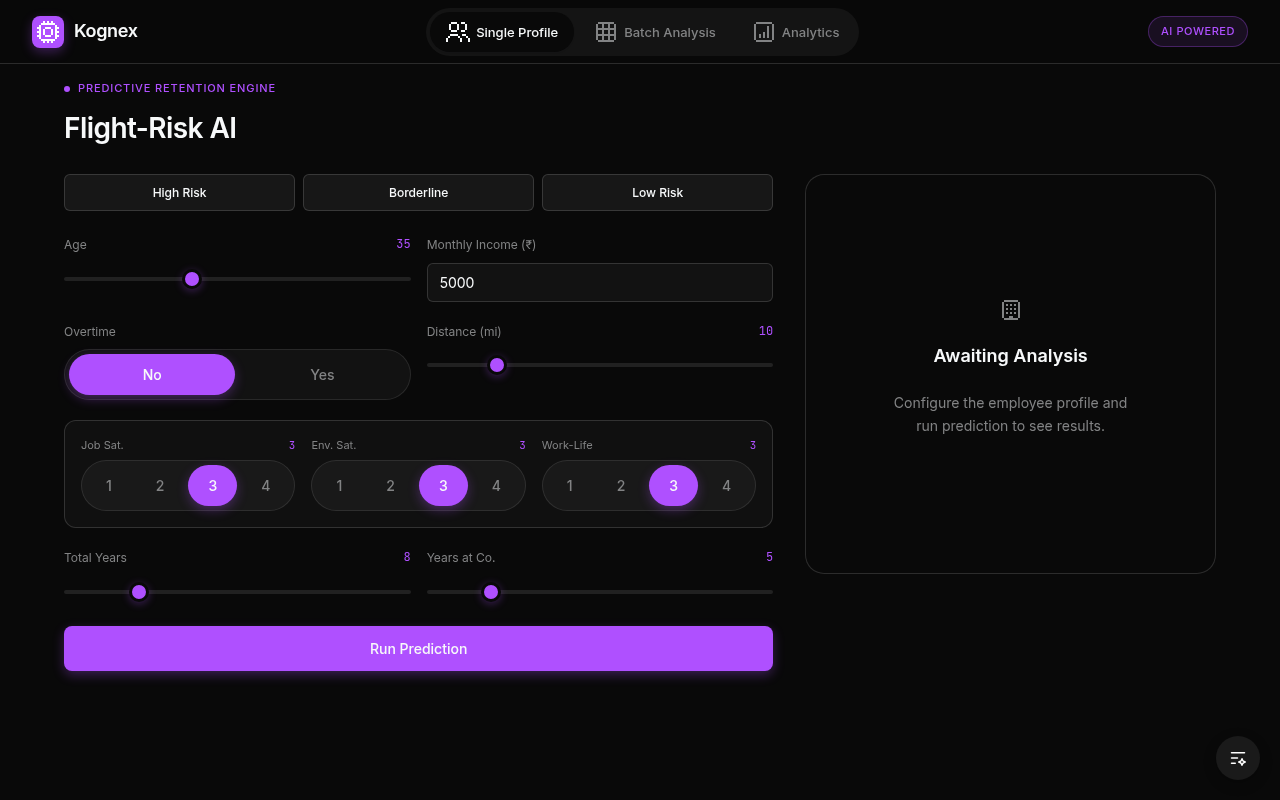
\includegraphics[width=0.9\linewidth]{figures/actual_app_screenshot.png}
    \caption{The Kognex Web Interface: Midnight Terminal Aesthetic}
    \label{fig:web_app}
\end{figure}

The deployed UI leverages the "midnight terminal" aesthetic detailed in Chapter 4. By inputting an employee's data points via the interface controls, the user instantly receives a calculated attrition probability. The interface is designed to highlight critical alerts using the brand's signature \texttt{\#af50ff} (Signal Violet) color against the dark canvas, ensuring that high-risk employees immediately draw the attention of the HR user, thereby fulfilling the project's objective of enabling proactive, targeted retention interventions.
